\section{Estado del arte / Marco teórico}
\subsection{Estado del arte}
\subsubsection{A multi-label classification method combined with texture enhancement for deepfake face detection}
\textcite{Deng2025} proponen el modelo Q2L-DeepFake, el cual busca extender la detección tradicional binaria hacia una clasificación multi-etiqueta para identificar manipulaciones en zonas específicas del rostro. La arquitectura utiliza una CNN (ResNet101) con un módulo enfocado a mejorar las texturas para identificar detalles sutiles en capas superficiales, la cual se conecta a un Transformer Decoder encargado de realizar la detección de falsificaciones mediante las etiquetas mencionadas anteriormente. Finalmente, integran la función de pérdida APL (Asymmetric Polynomial Loss) para manejar el desequilibrio entre clases y el balance de los datos.
Para la fase de entrenamiento, los autores mencionan la limitante que tuvieron debido a que los datos están pensados más en la clasificación binaria por lo que utilizaron el conjunto de datos Seq-Deepfake aplicando un preprocesamiento para redefinir las etiquetas características del rostro dividiéndolas en 5 categorías: cejas, nariz, labios, ojos y cabello. Con esto, lograron habilitar el aprendizaje multi-etiqueta, ampliando el nivel de distinción del modelo. De igual forma, el estudio fundamenta que la inclusión de un modelo de mejora de texturas es necesaria, debido a que los rastros de falsificación son en su mayoría imperceptibles y se encuentran comúnmente en las frecuencias altas y la información de textura de la imagen, su modelo actúa en las capas superficiales para extraer y amplificar residuos de textura antes de que la red abstraiga la información.

\subsubsection{Desarrollo de una aplicación Web con machine learning para la detección de Deepfakes en casos de suplantación de identidad digital}
\textcite{Yagual2024} utiliza técnicas de Machine Learning para reducir los riesgos de la suplantación de identidad digital generados por los Deepfakes. En su propuesta se desarrolla una aplicación web orientada a garantizar la seguridad digital, permitiendo que usuarios sin un conocimiento previo o especializado puedan analizar imágenes (en formatos como JPG, PNG o TIFF) para confirmar su veracidad.

El autor entrena un modelo mediante TensorFlow y Keras, empleando una Red Neuronal Convolucional (CNN). Esta arquitectura es utilizada para procesar la retícula de la imagen y extraer características faciales complejas, permitiendo al sistema identificar inconsistencias imperceptibles para el ojo humano. El modelo final aplica una clasificación binaria tradicional, priorizando la accesibilidad y la prevención del fraude sobre la complejidad arquitectónica.
\subsubsection{Deepfake Image Detection: A Review of Existing Methods and a Hybrid CNN-Based Proposed Framework}
En esta investigación, los autores \parencite{Tiwari2025} realizan una revisión de las limitantes actuales en la detección de Deepfakes, destacando problemas como el sesgo en los conjuntos de datos y la falta de generalización en escenarios reales. Para reducir dichas limitantes, proponen una arquitectura híbrida basada en una CNN que integra ResNet-50 (enfocada principalmente en bloques residuales) para realizar una extracción amplia de las características profundas, conectada a una red VGG-16 que funciona como un clasificador especializado.

Utilizan pesos pre-entrenados de ImagNet para ambas redes y diseñan una estrategia de entrenamiento en dos fases: primero, congelan las capas inferiores de VGG-16 (encargadas de detectar patrones visuales simples como bordes) para ajustar solamente las capas superiores utilizando las características extraídas por ResNet; posteriormente, realizan un proceso de fine-tuning selectivo en las capas superiores de ResNet-50 junto con el clasificador para especializar el sistema en la detección de artefactos de manipulación. Este enfoque, validado sobre los conjuntos de datos Celeb-DF y DFDC, busca equilibrar la capacidad de extracción de características locales profundas con una clasificación más eficiente, dando mayor importancia al tamaño de la arquitectura del modelo frente a procesos comunes como la compresión y el redimensionamiento.

\subsubsection{Digital Forensics Method for Fake Images Detection Using GAN Algorithm}
\textcite{Mashhadani2025} presentan un método de detección usando técnicas forenses basado en marcas de agua y contenido de imágenes falsas generadas con redes GAN, específicamente usando StyleGAN2-ADA. Se propone un flujo donde se toman imágenes, se redimensionan a 256 × 256 píxeles y se les inserta texto invisible de 5,000 caracteres mediante dos técnicas, bit menos significativo y transformada discreta del coseno, luego esas imágenes con marca de agua se utilizan como insumo para generar imágenes sintéticas con StyleGAN2-ADA en un entorno tipo Google Colab con GPU.

Realizan un análisis del impacto de las marcas de agua, la efectividad para detectar falsificación al extraer el texto oculto, reportando que el texto extraído desde las imágenes falsas se vuelve inentendible porque StyleGAN2-ADA altera el contenido, finalmente, se entrena un modelo de aprendizaje profundo basado en capas de convolución para clasificar imágenes como reales o falsas; los autores describen una arquitectura de varias capas y mencionan el uso de transformaciones de entrenamiento para mejorar la capacidad de generalizar.

Los autores refuerzan la importancia de pasar de una decisión global (real/falso) a una localización espacial mediante una  máscara binaria, además, al remarcar que ciertos enfoques requieren la imagen original y que, en su ausencia, disminuye la precisión, indica que un sistema debería operar sin referencia, apoyándose en huellas provenientes del contenido alterado.

\subsubsection{The Cat and Mouse Game: The Ongoing Arms Race Between Diffusion Models and Detection Methods}
\textcite{Laurier2024} presentan una revisión sobre la carrera armamentista entre la generación de imágenes mediante modelos de difusión y las técnicas de detección, y organizan el campo mediante una taxonomía de enfoques: análisis en dominio de frecuencia (p. ej., métodos basados en Fourier y en wavelets), análisis en dominio espacial (estadísticas locales, patrones de ruido y artefactos a nivel píxel), métodos de detección basados en aprendizaje profundo (redes neuronales convolucionales, transformadores de visión y detectores multimodales) y enfoques híbridos que combinan señales espaciales y frecuenciales; además, incorporan el rol de conjuntos de datos y bancos de prueba, así como implicaciones y aplicaciones relacionadas con desinformación, derechos de autor y análisis forense. 

Se discuten desafíos centrales que explican por qué la detección es un problema en evolución constante: los detectores suelen fallar al generalizar entre distintos modelos de difusión por la presencia de huellas específicas de cada generador, y también pierden desempeño ante transformaciones comunes en escenarios reales como compresión y redimensionamiento; adicionalmente, se subraya el caso de contenido mixto (elementos reales y sintéticos dentro de una misma imagen, como en tareas de relleno o secciones manipuladas), donde métodos globales pueden pasar por alto alteraciones locales y se requiere evaluar y diseñar métodos con capacidad de operar a nivel más fino, apoyados por conjuntos de datos más diversos que contemplen condiciones de uso real y protocolos de evaluación comparables.

Los autores señalan que en imágenes con contenido real y sintético mezclado es necesario distinguir componentes reales y generados dentro de la misma imagen, y proponen que esto se evalúe a nivel píxel, además de mencionar que se investigan técnicas de localización con supervisión débil para abordar este escenario; también enfatizan que los detectores deben ser robustos a compresión y reescalado (degradaciones comunes en redes sociales) y capaces de generalizar a modelos no vistos.

\subsection{Marco teórico}

\subsubsection{Manipulación facial y deepfakes}

\medskip\textbf{Definición operativa y tipología de manipulación facial}

\textcite{Mirsky2021} describen los deepfakes como contenido multimedia sintético o manipulado mediante técnicas de inteligencia artificial, donde la similitud visual se logra por modelos generativos capaces de reproducir rasgos faciales, texturas y patrones de iluminación con alta fidelidad. En el ámbito de visión por computadora, el término se utiliza de forma operativa para referirse a manipulaciones que alteran la identidad aparente o la dinámica facial de una persona, con o sin una fuente real de referencia, y que pueden integrarse a flujos de edición que ocultan rastros evidentes mediante posprocesamiento, por ejemplo, compresión y reescalado.

En particular, la manipulación facial puede organizarse como un conjunto de transformaciones sobre el rostro que abarcan:
\begin{itemize}
    \item Reemplazo de rostro (intercambio de identidad)
    \item Recreación o reenactment (transferencia de expresiones o movimientos faciales de un sujeto mediante las señales de otro)
    \item Edición (modificaciones localizadas del rostro sin sustituir por completo la identidad)
    \item Síntesis (generación de un rostro completo sin un objetivo real como base). 
\end{itemize}

Esta clasificación es importante porque describe que se espera encontrar: el reemplazo y la recreación tienden a introducir discontinuidades en contornos y coherencias internas del rostro, mientras que la síntesis puede producir coherencias globales altas, pero inconsistencias de textura en regiones específicas. \parencite{MurguiaSerrano2025}


Los flujos de generación y edición de rostros suelen incluir etapas de detección y alineación facial, extracción de representaciones (por ejemplo, puntos faciales o descriptores aprendidos), generación mediante modelos como redes generativas antagónicas (GAN) o modelos de difusión, y finalmente una fase de mezclado y posprocesamiento para integrar el rostro manipulado con el contexto (color, grano, compresión y bordes). La bibliografía indica que estas etapas no solo producen una "imagen falsa", sino que también pueden dejar huellas residuales de naturaleza local (texturas, microbordes, patrones de ruido o inconsistencias de iluminación) que son el objetivo de los detectores modernos. 

\medskip\textbf{Imagen alterada versus región alterada: implicaciones para la formulación del problema}

Una distinción clave para fines forenses es separar el caso de imagen alterada (una decisión global real/falsa) del caso de región alterada (alteración parcial dentro de la misma imagen). En escenarios reales, una manipulación puede afectar solo ciertas zonas del rostro y, además, las huellas pueden aparecer de forma no uniforme o en ubicaciones variables; por lo que hay una necesidad de detectar y localizar las áreas manipuladas, ya que la clasificación global puede pasar por alto alteraciones pequeñas o mezcladas con contenido real. Esta diferencia es especialmente importante cuando se busca producir evidencia visual verificable y no solo una etiqueta. 

\subsubsection{Detección de deepfakes: enfoques y taxonomía}

\medskip\textbf{Enfoques espacial, de frecuencia y aprendizaje profundo end-to-end}


La detección de deepfakes se ha consolidado como un problema central del análisis forense digital debido a la rápida evolución de los generadores y a la creciente dificultad para distinguir contenido real de contenido sintético bajo condiciones de despliegue reales. En este contexto, el propósito del presente apartado es ubicar la propuesta de esta tesis dentro del panorama del campo, identificando las familias de métodos dominantes, las señales que buscan explotar y las limitaciones estructurales que condicionan su vigencia, con especial énfasis en la generalización y en la degradación introducida por compresión y reescalado.

De forma operativa, la bibliografía organiza los enfoques de detección en función del tipo de evidencia que se modela y del espacio donde se manifiestan las huellas. En este trabajo se adopta una taxonomía de cuatro enfoques de alto nivel:
\begin{itemize}
    \item Enfoque espacial.
    \item Enfoque en frecuencia.
    \item Enfoque basado en aprendizaje profundo (end-to-end).
    \item Enfoques híbridos. 
\end{itemize}
Esta organización no pretende ser excluyente, ya que diversos modelos contemporáneos combinan señales y representaciones; sin embargo, permite sintetizar la intuición forense detrás de cada familia y, en consecuencia, discutir sus fallas típicas ante el cambio de dominio (conjunto de datos, generador y postprocesado) \parencite{MurguiaSerrano2025, Banerjee2025}.


En el enfoque espacial, la detección se apoya en inconsistencias observables en el dominio de píxel, es decir, irregularidades locales o globales que emergen del mezclado, la edición y la síntesis facial. Típicamente se buscan discontinuidades en contornos, incoherencias en iluminación, texturas atípicas, patrones de ruido residuales o discrepancias entre la región facial y su contexto. En implementaciones modernas, estas señales se capturan mediante extractores aprendidos (p. ej., CNN), que identifican patrones discriminativos asociados a manipulaciones y, en variantes orientadas a localización, habilitan mapas de activación o máscaras que aproximan la región alterada. No obstante, al depender de huellas que pueden ser atenuadas por posprocesamiento, su desempeño suele degradarse en escenarios con compresión, baja resolución u oclusiones, además de mostrar sensibilidad a sesgos de captura y a variaciones de escena. \parencite{Banerjee2025, Alrashoud2025}


En el enfoque de frecuencia, la hipótesis es que los procesos de generación introducen artefactos espectrales que no son necesariamente evidentes en el espacio de píxel, pero sí se manifiestan como anomalías en bandas de alta frecuencia o como distribuciones espectrales atípicas. Parte de la evidencia reportada en la bibliografía vincula estas huellas con operaciones internas de los generadores, por ejemplo, etapas de sobremuestreo en arquitecturas GAN, que dejan patrones característicos en el espectro. En consecuencia, se utilizan transformadas (p. ej., Fourier, DCT o wavelets) y descriptores espectrales para separar contenido real de contenido sintético. Sin embargo, una limitación crítica es que dichas huellas pueden variar entre generadores y, por tanto, inducir sobreajuste a patrones específicos del modelo de síntesis o del dominio de entrenamiento, reduciendo la capacidad de generalización a fuentes no vistas. \parencite{Tan2024}


El enfoque basado en aprendizaje profundo, entendido como detección end-to-end, agrupa estrategias donde el modelo aprende representaciones discriminativas directamente de los datos, sin depender explícitamente de un conjunto fijo de rasgos forenses diseñados a mano. En esta familia se incluyen arquitecturas CNN y variantes con mecanismos de atención o módulos complementarios, entrenadas en clasificación (real/falso) o en formulaciones que incorporan supervisión espacial cuando se dispone de anotaciones. Su ventaja práctica es la capacidad de modelar patrones complejos y no lineales; sin embargo, la bibliografía coincide en que el rendimiento reportado en pruebas intra-dataset no necesariamente se sostiene en evaluación cruzada entre conjuntos de datos, donde se presentan técnicas de falsificación no vistas, cambios de dominio y una distribución distinta a la del entrenamiento. En este sentido, la generalización se reconoce como un problema crítico, debido a la tendencia de muchos detectores a capturar correlaciones espurias o "huellas" específicas del generador, más que indicios robustos y transferibles. \parencite{Li2025, Yang2025}


\medskip\textbf{Enfoques híbridos y dinámica adversarial generador-detector}
Los enfoques híbridos surgen como respuesta directa a la fragilidad de un único tipo de evidencia. De manera general, un enfoque híbrido integra representaciones espaciales y espectrales, o combina señales forenses (p. ej., inconsistencias de compresión o señales residuales) con características aprendidas por redes profundas, mediante arquitecturas multirrama y mecanismos de fusión. La intuición es que la manipulación deja rastros en múltiples niveles: algunos son locales en el píxel, otros se expresan como firmas en frecuencia y otros se manifiestan como discrepancias de coherencia global; por lo tanto, la combinación explícita puede aumentar sensibilidad y robustez ante variaciones. En la bibliografía reciente se observa un énfasis en modelar interacciones espacio–frecuencia y en diseñar estrategias orientadas a mejorar la generalización, precisamente porque los artefactos aislados tienden a perder estabilidad frente a generadores nuevos y frente a interferencia por postprocesado. \parencite{Li2025, Qiao2025}


\medskip\textbf{Generalización y degradación por postprocesamiento}


El fenómeno de "gato y ratón" entre generadores y detectores describe una dinámica adversarial: a medida que los modelos de síntesis incrementan realismo y reducen artefactos visibles, los detectores deben migrar hacia señales más sutiles o hacia estrategias de entrenamiento que no dependan de firmas específicas. En consecuencia, un detector entrenado sobre una familia de manipulaciones puede experimentar degradación notable al enfrentarse a falsificaciones no vistas, lo cual limita la vigencia práctica de métodos altamente especializados. Esta dinámica también se relaciona con la necesidad de protocolos de evaluación más representativos y con el uso de bancos de prueba estandarizados que reflejen condiciones reales de circulación de contenido, donde cambian estilos, fuentes y procesos de compresión y reempaquetado. \parencite{Alrashoud2025, Chandra2025, Qiao2025}


 

En este marco, la generalización se entiende como la capacidad del detector para mantener desempeño ante cambios de dominio: nuevos generadores, nuevas distribuciones de datos y nuevas condiciones de captura y publicación. La evidencia reciente subraya que, incluso cuando los modelos obtienen resultados altos en conjuntos académicos, su desempeño puede caer de forma pronunciada en datos "in-the-wild", recolectados de plataformas y escenarios contemporáneos. Adicionalmente, la compresión, el reescalado y otros posprocesos actúan como perturbaciones que suprimen o distorsionan huellas forenses, afectando tanto señales espaciales (pérdida de microtextura) como señales espectrales (alteración de distribuciones de frecuencia). Por ello, la delimitación del problema hacia la localización/segmentación en la región facial de interés y la producción de evidencia visual (máscara y overlay) se alinean con la necesidad de ofrecer una salida verificable, aun cuando la decisión de clasificación global sea insuficiente en escenarios de alteración parcial. \parencite{Hu2024, Li2025, Chandra2025}

\subsubsection{Clasificación global vs localización}

\medskip\textbf{Limitaciones de la clasificación global ante manipulaciones locales}

La detección de deepfakes se puede tratar como un problema de clasificación global; este método es más tradicional, en donde un modelo asigna una etiqueta binaria (real/falso) a la imagen completa. El modelo aprende patrones estadísticos globales que distinguen imágenes auténticas de manipuladas. Si bien esta metodología es útil cuando la alteración afecta la imagen de forma general, suele tener limitaciones importantes en escenarios reales, donde las manipulaciones suelen ser locales o parciales.

En la práctica, muchas alteraciones digitales modifican únicamente regiones específicas del rostro —por ejemplo, ojos, boca o contornos faciales— mediante técnicas de reemplazo, reenactment o blending. Cuando la alteración está espacialmente restringida, los modelos de clasificación global pueden no detectar señales suficientemente discriminativas, especialmente después de procesos de poscompresión o suavizado que reducen los artefactos visibles. Esto puede derivar en falsos negativos, ya que la imagen conserva gran parte de su estadística global intacta.

\begin{figure}[H]
    \centering
    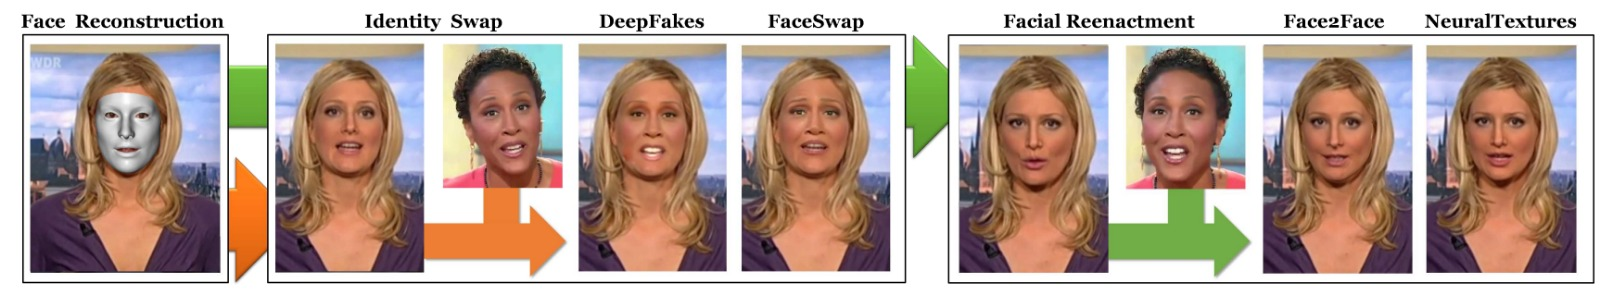
\includegraphics[width=\textwidth]{imagenes/Analisis_clasificación_binaria.jpeg} 
    \caption{Ejemplos de manipulaciones faciales empleadas en la generación de deepfakes. Se observan técnicas como reemplazo de rostro (DeepFakes, FaceSwap), reenactment (Face2Face) y restauración (Face Restoration, Neural Textures). Estas alteraciones suelen concentrarse en áreas localizadas (ojos, boca, contornos), lo que justifica el uso de métodos de segmentación en lugar de clasificación global.}
    \label{fig:tipos_manipulaciones}
\end{figure}

\medskip\textbf{Reformulación como tarea de localización y valor forense del overlay}


Por esta razón, el problema abordado en este trabajo se reformula como una tarea de localización de manipulación, donde el objetivo no es únicamente determinar si una imagen es falsa, sino identificar qué regiones específicas han sido alteradas. En lugar de producir una etiqueta global, el modelo genera un mapa espacial o máscara que asigna a cada píxel una probabilidad de pertenecer a una zona manipulada. Esta metodología permite que el uso de la segmentación semántica modele con precisión la estructura espacial donde se realizó una alteración.

La generación de una máscara (overlay) aporta además un valor técnico y forense significativo: proporciona evidencia visual interpretable, permite cuantificar la extensión de la manipulación (porcentaje de píxeles afectados) y facilita análisis posteriores centrados exclusivamente en las regiones sospechosas. Por otra parte, el uso de una clasificación global no aporta esta información, lo que puede producir falsos negativos, haciendo nulo su valor como herramienta forense y disminuyendo progresivamente su efectividad.

\begin{figure}[H]
    \centering
    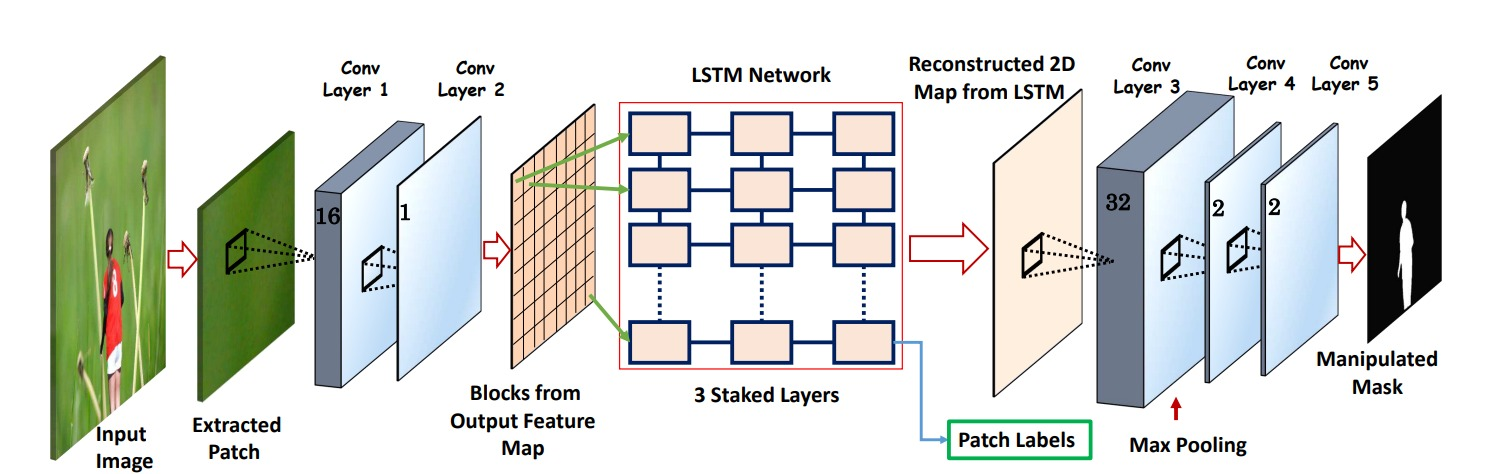
\includegraphics[width=\textwidth]{imagenes/Analisis_pixel.jpeg} 
    \caption{Arquitectura de red neuronal convolucional para localización de manipulaciones. La imagen de entrada se procesa mediante capas convolucionales (Conv Layer 1-5) que extraen características multiescala. Luego, bloques LSTM modelan dependencias espaciales y finalmente se genera una máscara binaria (manipulated mask) que identifica las regiones alteradas a nivel de píxel. Este enfoque permite no solo detectar la falsificación, sino también delimitar su extensión espacial.}
    \label{fig:arquitectura_localizacion}
\end{figure}

\medskip\textbf{Criterio de evaluación espacial y métricas de segmentación}

Diversos trabajos como los estudios basados en el dataset FaceForensics++, muestran que los detectores globales pueden mantener un buen desempeño en escenarios controlados, pero pierden su eficiencia  frente a manipulaciones localizadas, contenido mixto o degradaciones introducidas por compresión \parencite{Rossler_2019_ICCV}. En consecuencia, investigaciones recientes incorporan explícitamente tareas de localización y generación de mapas de manipulación como parte fundamental del análisis forense automatizado. \parencite{Bappy_2017_ICCV}

Bajo esta perspectiva, la presente investigación adopta un enfoque de segmentación píxel a píxel, donde la precisión del modelo se evalúa mediante métricas espaciales identificando así, para cada píxel generado por el modelo, la probabilidad de que sea alterado o no.

\subsubsection{Fundamentos de CNN para visión por computadora}


\medskip\textbf{Redes neuronales convolucionales}


\textcite{goodfellow2016deep} describen las redes neuronales convolucionales como un tipo de red neuronal specializada en el procesamiento de datos que tiene una topología conocida similar a una cuadrícula. Mencionan particularmente a las imágenes, las cuales pueden considerarse como una cuadrícula bidimensional de píxeles. El nombre "red neuronal convolucional" indica que la red emplea una operación matemática llamada convolución. La convolución es un tipo specializado de operación lineal. Por su parte las redes neuronales convolucionales son simplemente redes neuronales que utilizan la convolución en lugar de la multiplicación matricial general en al menos una de sus capas. 


\medskip\textbf{La operación de convolución}


La operación de convolución se define como una operación matemática entre dos funciones que produce una tercera función que representa la cantidad de superposición entre ellas. En términos continuos puede expresarse como:
 
\[
    s(t) = \int x(a)w(t - a)da
\]
Esta operación se denomina convolución y normalmente se indica con un asterisco 
\[
s(t)=(x*w)(t)
\]
Donde:
\begin{itemize}
    \item 	x representa la señal de entrada o los datos originales. En el contexto de las redes neuronales convolucionales, esta señal corresponde a los valores de los píxeles de una imagen
    \item 	w representa el filtro o kernel de convolución en el contexto de CNN el cual es una matriz de valores que se utilizan para detectar características específicas en la imagen (Bordes, texturas, patrones, etc.)
    \item 	* representa la operación de convolución entre la señal de entrada x y el filtro w
    \item 	t representa la posición o desplazamiento en la señal o imagen donde se está aplicando el filtro
    \item 	s(t) es el resultado de la convolución, es decir, una señal nueva resultante del proceso de convolución o un mapa de activación en el contexto de las CNN obtenido después de aplicar un filtro a una señal de entrada.
\end{itemize}


En el contexto de redes neuronales convolucionales, esta operación se utiliza para aplicar filtros sobre imágenes con el objetivo de detectar patrones locales como bordes, texturas o formas. Cada filtro se desplaza sobre la imagen generando mapas de activación que resaltan dichas características.

Sin embargo, en aplicaciones de aprendizaje automático y visión por computadora, los datos utilizados no son continuos sino discretos. Las imágenes digitales, por ejemplo, se representan como matrices de valores numéricos correspondientes a píxeles. Debido a esto, la operación de convolución se expresa mediante una forma discreta, en la cual la integral es reemplazada por una suma.

\[
s(t)=\sum_a x(a)w(t-a)
\]
Donde: 
\begin{itemize}
    \item x(a) representa la señal de entrada en la posición a
    \item w(t-a) valor del filtro desplazado 
    \item a representa el índice discreto de la suma 
    \item s(t) es el resultado de la convolución en la posición t 
\end{itemize}

Debido a que las imágenes digitales se pueden representar como matrices bidimensionales de píxeles, para llevar a cabo el proceso de convolución se aplica la misma fórmula, pero adaptada a dos dimensiones:
\[
s(i,j)=\sum_m\sum_n x(i-m,j-n)w(m,n)
\]
Donde: 
\begin{itemize}
    \item x(i,j) es el valor del píxel en la imagen de entrada.
    \item w(m,n) es el valor del filtro o kernel.
    \item s(i,j)  es el resultado de la convolución en la posición (i,j).
    \item m,n son los índices del kernel.
\end{itemize}

\begin{figure}[H]
    \centering
    
\includegraphics[width=0.5\linewidth]{Ejemplo_convolucion_2_dimensiones.png}
    \caption{Ejemplo de un proceso de convolución en una matriz de 2 dimensiones y el proceso para generar cada uno de los elementos (tensores) que componen el mapa de activación resultante después de aplicar el filtro en la matriz de entrada}
    \label{fig:convolucion_2d}
\end{figure}

Aunque el término convolución es ampliamente utilizado en redes neuronales convolucionales, en la práctica la operación implementada en la mayoría de los frameworks de aprendizaje profundo corresponde técnicamente a una correlación cruzada (cross-correlation). La principal diferencia entre ambas operaciones radica en que la convolución implica una inversión del filtro antes de realizar el desplazamiento sobre la señal de entrada, mientras que en la correlación el filtro se aplica directamente sin dicha inversión. A pesar de esta diferencia matemática, en el contexto del aprendizaje profundo ambos términos suelen utilizarse de manera intercambiable, ya que los filtros son aprendidos automáticamente durante el entrenamiento de la red.


\medskip\textbf{Filtros, mapas de activación y jerarquía de características.}


En las redes neuronales convolucionales, los filtros o kernels son pequeñas matrices de valores que se utilizan para detectar características específicas dentro de una imagen. Estos filtros se desplazan sobre la matriz de entrada aplicando la operación de convolución o correlación en cada posición. Durante el proceso de entrenamiento, los valores de los filtros se ajustan automáticamente mediante algoritmos de optimización, permitiendo que la red aprenda a identificar patrones relevantes en los datos.


 


El resultado de aplicar un filtro sobre una imagen de entrada se denomina mapa de activación (feature map). Este mapa representa la respuesta del filtro en cada posición de la imagen, resaltando aquellas regiones donde el patrón detectado por el filtro está presente. Cada filtro genera un mapa de activación diferente, lo que permite a la red neuronal capturar múltiples características visuales dentro de la imagen.


Las redes neuronales convolucionales aprenden una jerarquía de características visuales a través de sus diferentes capas. En las primeras capas, los filtros suelen detectar características simples como bordes y orientaciones. En capas intermedias, la red comienza a identificar patrones más complejos como texturas o formas. Finalmente, en las capas más profundas se reconocen estructuras más complejas, como partes de objetos o configuraciones faciales completas. Esta capacidad de aprender representaciones jerárquicas permite a las CNN analizar imágenes de forma eficiente en tareas de reconocimiento y clasificación.
Esta capacidad resulta especialmente útil en la detección de deepfakes, ya que permite identificar inconsistencias visuales sutiles en imágenes manipuladas, tales como anomalías en texturas faciales, iluminación o patrones de compresión.


En las redes neuronales convolucionales, esta operación se aplica repetidamente a través de múltiples capas convolucionales. Cada capa utiliza varios filtros que son aprendidos automáticamente durante el proceso de entrenamiento, permitiendo a la red detectar diferentes tipos de características visuales. Como resultado, se generan múltiples mapas de activación que capturan patrones relevantes dentro de la imagen de entrada.


\medskip\textbf{Pooling y stride.}

En las redes neuronales convolucionales, el pooling es una operación mediante la cual se busca reducir la dimensionalidad o tamaño de los mapas de activación generados por las capas convolucionales. Esta reducción permite disminuir el número de parámetros que utiliza el modelo y el costo computacional, al mismo tiempo que se conserva la información más relevante para las características que anteriormente se detectaron. Este proceso consiste en dividir el mapa de activación en pequeñas regiones y aplicar una función de agregación sobre cada una de ellas dando como resultado un mapa de activación más pequeño que conserva las características más importantes detectadas por los filtros de la red.


El max pooling es uno de los métodos de pooling más utilizados en redes neuronales convolucionales. En este método, para cada región del mapa de activación se selecciona únicamente el valor máximo. De esta manera, se conserva la característica más significativa detectada por el filtro en esa región específica.
Este mecanismo permite que la red neuronal mantenga las activaciones más relevantes y reduzca la información irrelevante, lo que ayuda a mejorar la eficiencia del modelo.


Otro método utilizado es el average pooling, el cual calcula el valor promedio dentro de cada región del mapa de activación. Aunque este método también reduce la dimensionalidad de los datos, en la práctica el max pooling suele utilizarse con mayor frecuencia en arquitecturas modernas de redes neuronales convolucionales debido a su mejor desempeño en muchas tareas de visión por computadora.


En la operación de convolución, el stride (comúnmente traducido como paso o zancada) es un hiperparámetro estructural que determina la cantidad de unidades espaciales o píxeles que el filtro (kernel) avanza sobre la matriz de entrada en cada iteración.
En las operaciones de convolución estándar, se asume un desplazamiento unitario (stride = 1), lo que significa que el filtro se mueve un píxel a la vez de izquierda a derecha y de arriba hacia abajo, procesando la imagen de manera altamente superpuesta.
 Sin embargo, al incrementar este valor (por ejemplo, un stride de 2), el filtro "salta" posiciones, desplazándose de dos en dos píxeles.
El impacto principal del stride se ve reflejado en las dimensiones espaciales del mapa de activación resultante una vez terminado el proceso de convolución, si el stride es grande, las dimensiones serán menores, actuando como un mecanismo de submuestreo y se denota de la siguiente manera:
\[
O = \left\lfloor \frac{W - K + 2P}{S} \right\rfloor + 1
\]


Donde:
\begin{itemize}
    \item O representa la dimensión espacial del mapa de activación de salida
    \item W es la dimensión de la imagen o matriz de entrada
    \item K es el tamaño del filtro o kernel
    \item P representa el padding (relleno) aplicado a los bordes de la entrada
    \item S es el valor del stride o desplazamiento.
\end{itemize}
\medskip\textbf{Funciones de activación.}


En las redes neuronales convolucionales, después de realizar la operación de convolución, se aplica una función de activación. Estas funciones introducen no linealidad en el modelo, lo cual permite que la red neuronal pueda aprender representaciones más complejas de los datos. Sin la incorporación de funciones no lineales, una red compuesta únicamente por operaciones lineales sería equivalente a una sola transformación lineal, limitando significativamente su capacidad de aprendizaje.
Las funciones de activación se aplican a los valores generados por las capas convolucionales, produciendo mapas de activación que posteriormente son procesados por las siguientes capas de la red. De acuerdo con \textcite{goodfellow2016deep}, las funciones de activación permiten que las redes neuronales profundas modelen relaciones complejas presentes en los datos y facilitan el aprendizaje de representaciones jerárquicas en tareas de visión por computadora.

Una de las funciones de activación más utilizadas en redes neuronales convolucionales es la Rectified Linear Unit (ReLU). Esta función se caracteriza por su simplicidad y eficiencia computacional, ya que transforma los valores negativos en cero y mantiene los valores positivos sin modificación.

La función ReLU puede definirse como:

\[
f(x)=\max(0,x)
\]
Donde: 
\begin{itemize}
    \item x representa el valor de entrada proveniente de la capa convolucional
    \item f(x) corresponde al valor resultante después de aplicar la función de activación.
\end{itemize}
Según \textcite{goodfellow2016deep}, el uso de la función ReLU facilita el entrenamiento de redes neuronales profundas, ya que ayuda a reducir el problema del gradiente desvanecido y permite una convergencia más rápida durante el proceso de aprendizaje.

Aun con la eficiencia de ReLU en las capas ocultas para la extracción de características, la salid de la red ocupa un enfoque diferente, pues las clasificación binaria como la generación de mascaras en problemas de segmentación semántica mediante arquitecturas como U-Net \textcite{Ronneberger2015}, por ellos la salid del modela se interpreta como una probabilidad, la función de activación sigmoide, comprime el valor real de la de entrada en un intervalo continuo entre el 0 y 1 lo cual según \textcite{goodfellow2016deep} resulta determinante para calcular la probabilidad de pertenecer a una clase.

\begin{equation}
f(x) = \frac{1}{1 + e^{-x}}
\end{equation}

Donde $e$ representa la base del logaritmo natural.

\subsubsection{Segmentación semántica y formulación del problema.}

\medskip\textbf{Artefactos e inconsistencias en deepfake.}

El uso desmedido de redes generativas (GAN) para producir deepfakes ha conducido a una proliferación de imágenes y con ello, al aumento del realismo. Sin embargo, aún con todos estos avances se pueden detectar por las técnicas correctas artefactos visuales que delatan su intervención. “FaceForensics++: Learning to Detect Manipulated Facial Images de Andreas Rossler” demostró que aún existe irregularidades en textura de piel asi como iluminación y sombras.

Dentro del dominio contextual de un rostro, la mayor inconsistencia presente de texturas se presenta cuando se realiza un suavizado en la piel o bien cuando estén perdida de imperfecciones que la piel debería de conservar y más con los avances de calidad digital al momento de capturar contenido. Este tipo de efectos surgen cuando en la generación de la manipulación se le da prioridad a una coherencia global sobre las particulares detalladas (Ejemplo: Un tono de piel informe por sobre la generación de líneas de expresión) lo que provoca transiciones notorias entre el rostro alterado y la imagen real, las zonas que más se delatan son el cabello y el contorno facial. Otro tipo de incoherencia visual que se presenta con regularidad son la dualidad de sombra y luz que resaltan por no coincidir con la imagen real.

\medskip\textbf{Altas frecuencias y residuos de textura.}

Un aspecto para tomar en cuenta es el análisis de alta frecuencia, el cual suele abarcar información acerca de bordes, detalles fino o micro texturas. Los cuales se alteran durante la generación de un “deepfake”. Detección como el propuesto como “MesoNet: a Compact Facial Video Forgery Detection Network de Darius Afchar” mencionan que se puede tomar ventaja de los residuos de textura para extraer características o rastros de manipulación. En varios casos la region manipulada presenta un conjunto de frecuencias distintas a las imágenes reales, permitiendo detección que serían difícil para la percepción del ojo del ser humano 

\medskip\textbf{Segmentación semántica.}

Las técnicas de segmentación semántica permiten asignar una etiqueta a cada píxel de una imagen según su contexto. A diferencia de un método tradicional de clasificación que genera una etiqueta global, la segmentación permite determinar ubicación dentro las imágenes, dicho enfoque resulta útil en un análisis forense permitiendo la localización espacial.

\begin{figure}[H]
\centering

\includegraphics[width=0.9\textwidth]{Segmentacion_semantica.jpg}
\caption{Ejemplo de segmentación semántica. A la izquierda se muestra la imagen original y a la derecha el mapa de segmentación donde cada píxel es clasificado en una categoría semántica distinta.}
\label{fig:segmentacion_semantica}
\end{figure}

Como se observa en la Figura \ref{fig:segmentacion_semantica}, la segmentación semántica permite identificar diferentes regiones dentro de una imagen mediante etiquetas asignadas a cada píxel. En este proyecto, en lugar de múltiples categorías semánticas, el objetivo consiste en distinguir únicamente entre regiones manipuladas y regiones auténticas dentro del rostro.

\medskip\textbf{Formulación del problema como segmentación binaria.}

El objetivo del modelo es aprender una función que a partir de una imagen del rostro pueda generar un mascara binaria que indique regiones manipuladas, De esta forma los pixeles pertenecientes a una clase se pueden representar asignándole el calor 0, caso contrario los pixeles con de regiones de otras clases se podrá asignar el valor 1. Dicho formulación permitirá localizar con precisión las áreas de la alteración.